%***************************************PREAMBLE***************************************
\documentclass[a4paper,12pt]{article}

\usepackage[utf8]{inputenc}
\usepackage[margin=0.7in]{geometry}
\usepackage[T1]{fontenc}
\usepackage{graphicx}
\usepackage{float}
\usepackage{setspace}
\usepackage{appendix}

\usepackage{caption}
\usepackage{subcaption}

%***************************************DOCUMENT***************************************

\begin{document}
	\fontfamily{ptm}\selectfont
	%%%%%%%%%%%%%%%%%%%%%%%%%%%%%%%%%%%%%%%COVERSHEET%%%%%%%%%%%%%%%%%%%%%%%%%%%%%%%%%%%%%%%
	\begin{titlepage}
		\setlength{\voffset}{-0.8in}
		\noindent \makebox[\textwidth]{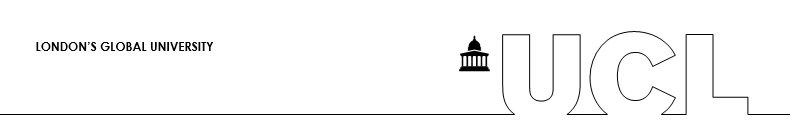
\includegraphics[width=1.2\textwidth]{images/Coversheet_Header.png}}
	
			\vspace{15mm}
			
			\begin{center}
				{\Huge \textbf{COMP0037 \\ \vspace{10mm} Report}}
			
				\vspace{8mm}
			
				\begin{spacing}{1.8}
					{\huge Exploration in Unknown Environments}
				\end{spacing}
		
			
				\vspace{12mm}
			
				{\LARGE \textbf{Group AS}}
				
				\vspace{10mm}
				
				\begin{tabular}{ll}
					\underline{\textbf{Student Name}}  & \hspace{4mm} \underline{\textbf{Student number}} \vspace{2mm} \\
					Arundathi Shaji Shanthini & \hspace{4mm} 16018351 \\ 
					Dmitry Leyko & \hspace{4mm}  16021440\\ 
					Tharmetharan Balendran & \hspace{4mm} 17011729\\ 
				\end{tabular}
				
				\vspace{13mm}
				
				\begin{tabular}{ll}
					\textbf{Department:} &  Department of Electronic and Electrical Engineering\\ \vspace{3mm}
					\textbf{Submission Date:} &  17\textsuperscript{th} of March 2020
				\end{tabular}
			\end{center}
	\end{titlepage}
	%%%%%%%%%%%%%%%%%%%%%%%%%%%%%%%%%%%%%%
	
	\pagebreak
	
	\tableofcontents
	
	\pagebreak
	
	%%%%%%%%%%% PART 1 %%%%%%%%%%%%%%%%%
	\section{Reactive Planner }
		\begin{figure}[H]
			\centering
			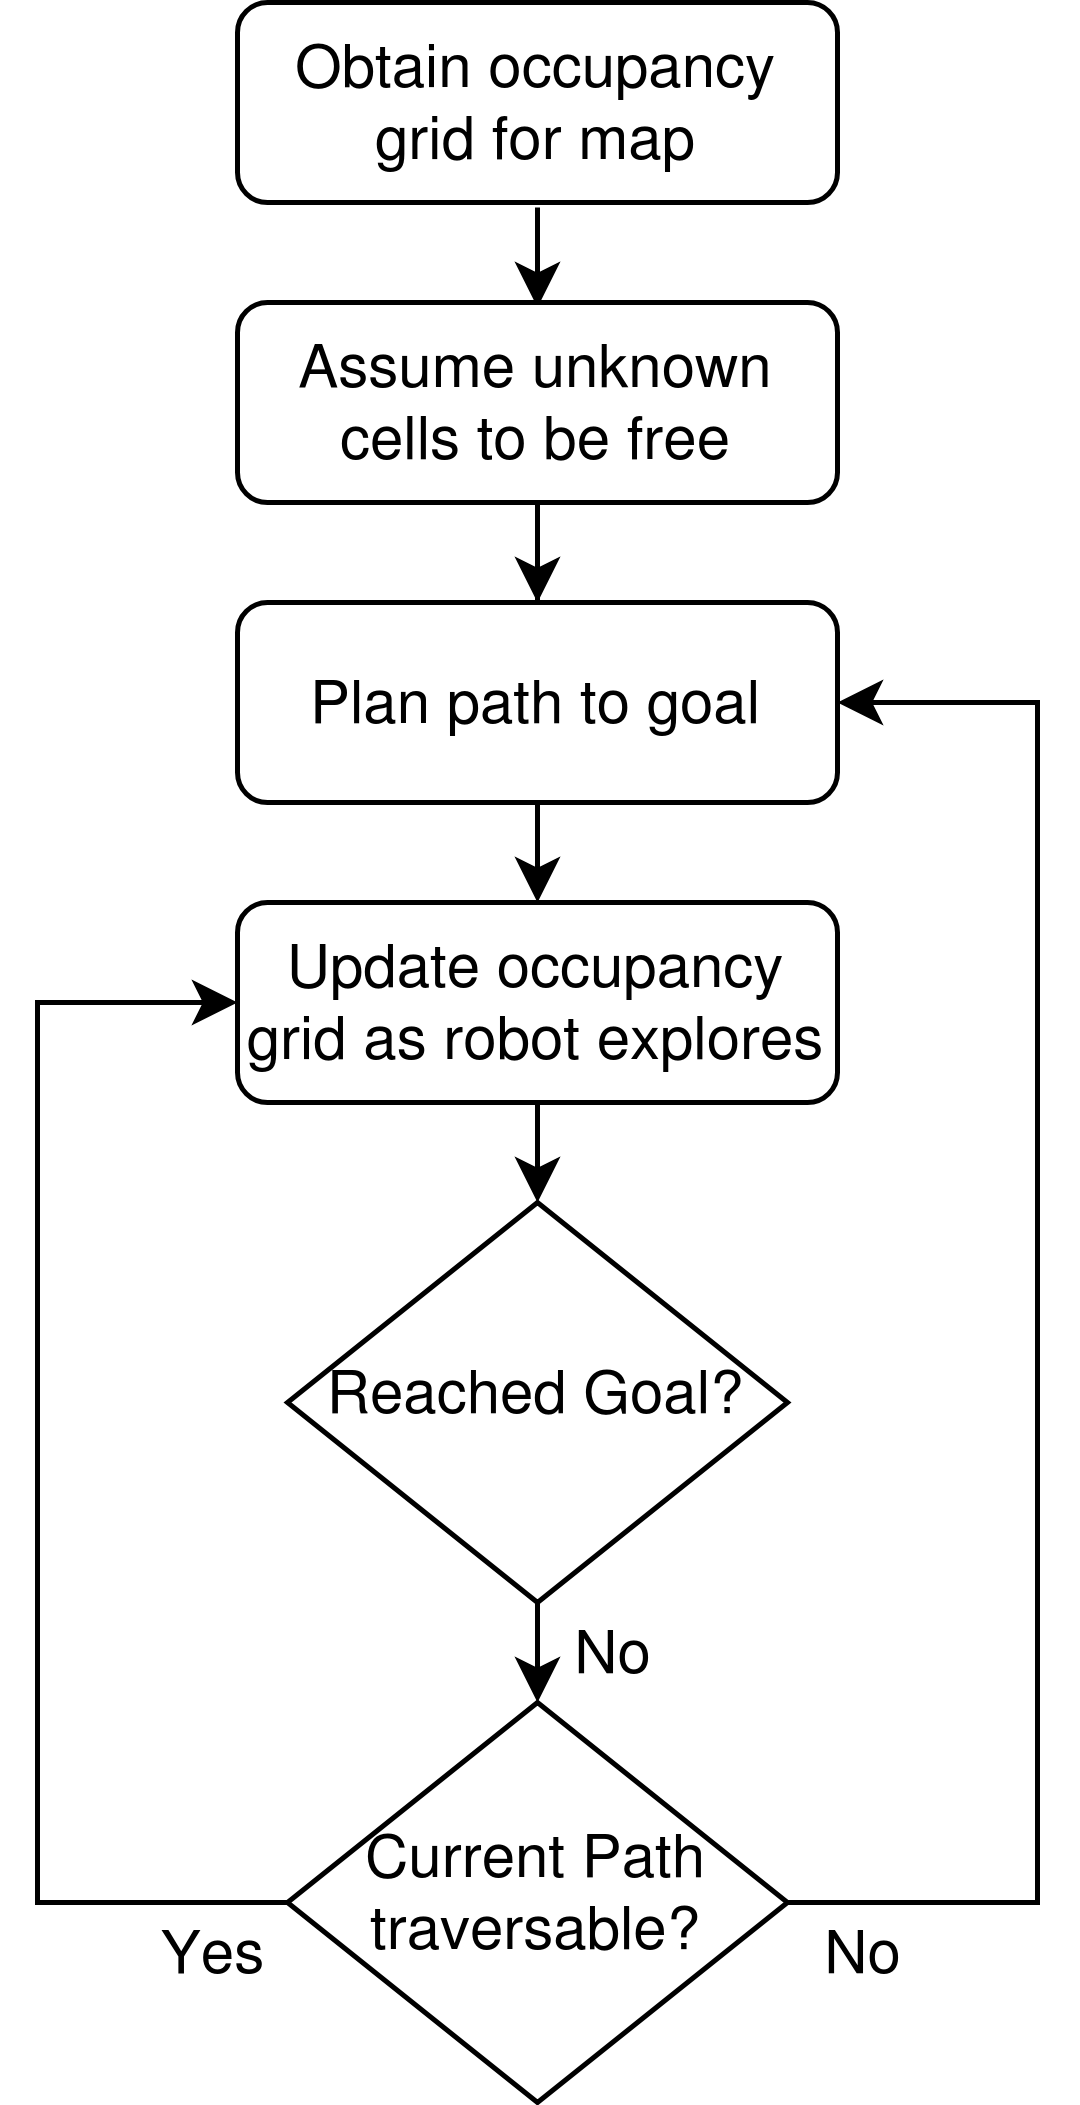
\includegraphics[scale=0.15]{images/reactivePlannerFlowchart.png}
			\caption{Flowchart for the reactive planner}
			\label{reactivePlannerFlowchart}
		\end{figure}
	
		\subsection{Our Implementation of a Reactive Planner}

			A reactive planner is able to adapt its path based on the information it obtains about the environment as it explores it. The high-level functionality of a general reactive planner is described in the flowchart in Fig.\ref{reactivePlannerFlowchart}. The reactive planner initially utilizes the available occupancy grid and assumes any unknown cells to be free. The planner then plans a path using this assumption and starts to traverse the path. The robot will explore the environment as it traverses the path and if new information suggests that the currently planned path is no longer traversable, a new path is planned using the new occupancy grid. This process is repeated until the robot arrives at the goal.
			\\
			As a means of testing the code the robot was set to visit a list of goals on the factory map. The final mapper node occupancy grid is shown in Fig.\ref{mapperNodeOccupancyGrid}. It is clear to see that there are inaccuracies in the mapping of the world as well as some areas which have still not been explored completely. The inaccuracies occur as a result of rounding errors and other noise due to timing mismatch (caused by networking delays), these errors are mostly corrected as the robot re-explores an area.
			\\
			The way the map is updated is using the laser range finder that the robot is equipped with. Depending on the reflections of this laser, the environment surrounding the robot can be mapped. Fig.\ref{robotLaserRange} depicts an instance in time of the robot. The red lines represent the individual laser beams used to map the surrounding environment. It is clear to see that the laser beam is stopped (and reflected) by the opaque walls. By measuring the time taken for the reflected beam to return, the distance to the opaque object can be calculated. In addition to this, it can also be seen that some of the beams stop despite not having hit any opaque objects. This is due to the maximum measurable range of the laser range detector. 

			\begin{figure}[H]
				\centering
				\begin{subfigure}{.5\textwidth}
				\centering
				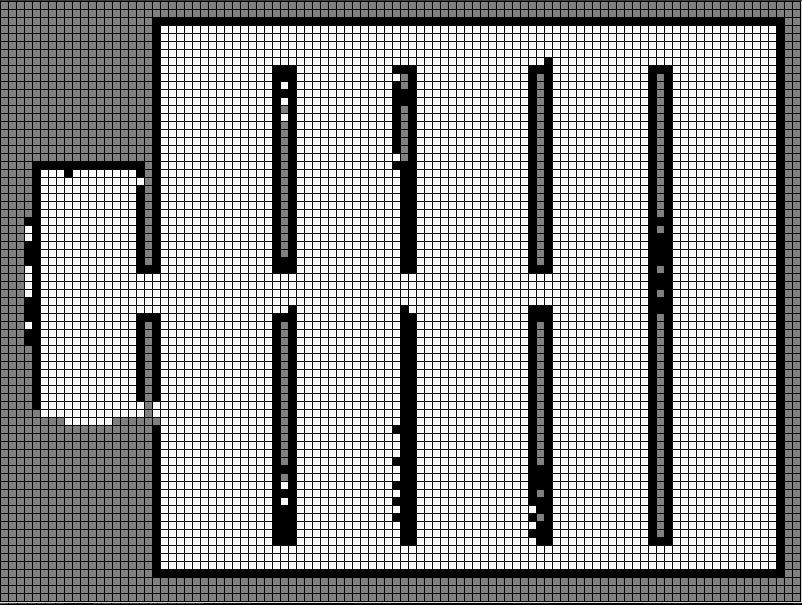
\includegraphics[width=.7\linewidth]{images/mapperNodeOccupancyGrid.png}
				\caption{Mapper Node occupancy grid}
				\label{mapperNodeOccupancyGrid}
				\end{subfigure}%
				\begin{subfigure}{.5\textwidth}
				\centering
				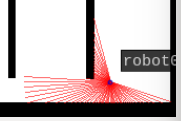
\includegraphics[width=.7\linewidth]{images/robotLaserRange.png}
				\caption{Robot Laser Range Finder}
				\label{robotLaserRange}
				\end{subfigure}
				\caption{a) Mapper occupancy grid at the end of traversing the set of goals. b) The robot traversing the map with the laser range finder visualized by the red lines. The maximum range as well as the opaque walls preventing the laser from passing through can also be seen.}
				\label{fig:test}
				\end{figure}

		\subsection{Improving the performance of the Reactive Planner}

		
	%%%%%%%%%%%%%%%%%%%%%%%%%%%%%%%%%%%%%%
	
	%%%%%%%%%%% PART 2 %%%%%%%%%%%%%%%%%
	\section{Frontier-Based Exploration System}
	
	
	%%%%%%%%%%%%%%%%%%%%%%%%%%%%%%%%%%%%%%
	
	%%%%%%%%%%% PART 3 %%%%%%%%%%%%%%%%%
	\section{Mapping the Environment}
	
	
	%%%%%%%%%%%%%%%%%%%%%%%%%%%%%%%%%%%%%%
	
	%%%%%%%%%%% PART 4 %%%%%%%%%%%%%%%%%
	\section{Information-Theoretic Path Planning}
	
	
	%%%%%%%%%%%%%%%%%%%%%%%%%%%%%%%%%%%%%%
	
	\newpage
	
	\appendix
	\appendixpage
	\addappheadtotoc
	
\end{document}